\section{Technique}

\begin{frame}
  \tableofcontents[currentsection,hideothersubsections]
\end{frame}


\begin{frame}[fragile]
  \frametitle{Wire Cell Reconstruction Method}
  \setbeamercovered{transparent}
  \begin{columns}
    \begin{column}{0.7\textwidth}
      Four main parts:
      \begin{enumerate}
      \item<2> Data Preparation
        \begin{itemize}        \scriptsize
        \item Deconvolve \textbf{detector response and filter noise}.
        \item Construct \textbf{wire} geometry and associated \textbf{cells}.
        \item Read framed data stream, form \textbf{time slices}
        \end{itemize}
      \item<3> Imaging of Activity
        \begin{itemize}        \scriptsize
        \item The heart of the Wire Cell technique
        \item Identify the likely hit \textbf{cells} in each time slice.
        \end{itemize}
      \item<4> Pattern Recognition 
        \begin{itemize}         \scriptsize
        \item Application of Wire Cell imaging
        \item \textbf{Cluster} activity in space and across time slices.
        \item \textbf{Categorize}: track, shower, etc.
        \end{itemize}
      \item<5> Physics Quantities
        \begin{itemize}         \scriptsize
        \item Determine particle ID and kinematics of tracks/showers.
        \end{itemize}
      \end{enumerate}
    \end{column}
    \begin{column}{0.3\textwidth}
      \begin{center}
        \vspace{-10mm}
        \resizebox{!}{\textheight}{
\begin{tikzpicture}[align=center, node distance=2cm]

\tikzstyle{dataobj} = [rectangle, rounded corners, minimum width=3cm, minimum height=1cm,text centered, draw=black, fill=blue!30]
\tikzstyle{process} = [rectangle, minimum width=3cm, minimum height=1cm, text centered, draw=black, fill=orange!30]
\tikzstyle{decision} = [diamond, minimum width=3cm, minimum height=1cm, text centered, draw=black, fill=green!30]
\tikzstyle{arrow} = [thick,->,>=stealth]

\node (daqmc) [process,highlight=2] {DAQ/MC sim};
\node (frames) [dataobj, below of=daqmc] {Stream Frames};
\node (slicing) [process,highlight=2, below of=frames] {Slicing};
\node (slices) [dataobj, below of=slicing] {Time Slices};
\node (wires) [dataobj, left=0.5cm of frames] {Wire geometry};
\node (tiling) [process,highlight=2, left=0.5cm of slicing] {Cell Tiling};
\node (cells) [dataobj, left=0.5cm of slices] {Cells geometry};
\node (hitcells) [process,highlight=3, below of=slices] {Hit cell selection};
\node (blobbing) [process,highlight=3, below of=hitcells] {Blob forming};
\node (clustering) [process,highlight=4, below of=blobbing] {Clustering};
\node (tracking) [process,highlight=4, below of=clustering] {Tracking};
\node (pid) [process,highlight=5, below of=tracking] {Particle ID};
\node (physics) [dataobj, below of=pid] {Physics Quantities};

\draw [arrow] (wires) -- (tiling);
\draw [arrow] (tiling) -- (cells);
\draw [arrow] (cells) -- (hitcells);
\draw [arrow] (daqmc) -- (frames);
\draw [arrow] (frames) -- (slicing);
\draw [arrow] (slicing) -- (slices);
\draw [arrow] (slices) -- (hitcells);
\draw [arrow] (hitcells) -- (blobbing);
\draw [arrow] (blobbing) -- (clustering);
\draw [arrow] (clustering) -- (tracking);
\draw [arrow] (tracking) -- (pid);
\draw [arrow] (pid) -- (physics);
\end{tikzpicture}}
      \end{center}
    \end{column}
  \end{columns}

\end{frame}

\subsection{Data Preparation}


\begin{frame}[fragile]
  \frametitle{Time Slicing}
  
  \begin{columns}
    \begin{column}{0.35\textwidth}
      \begin{center}
        \vspace{-.5cm}

        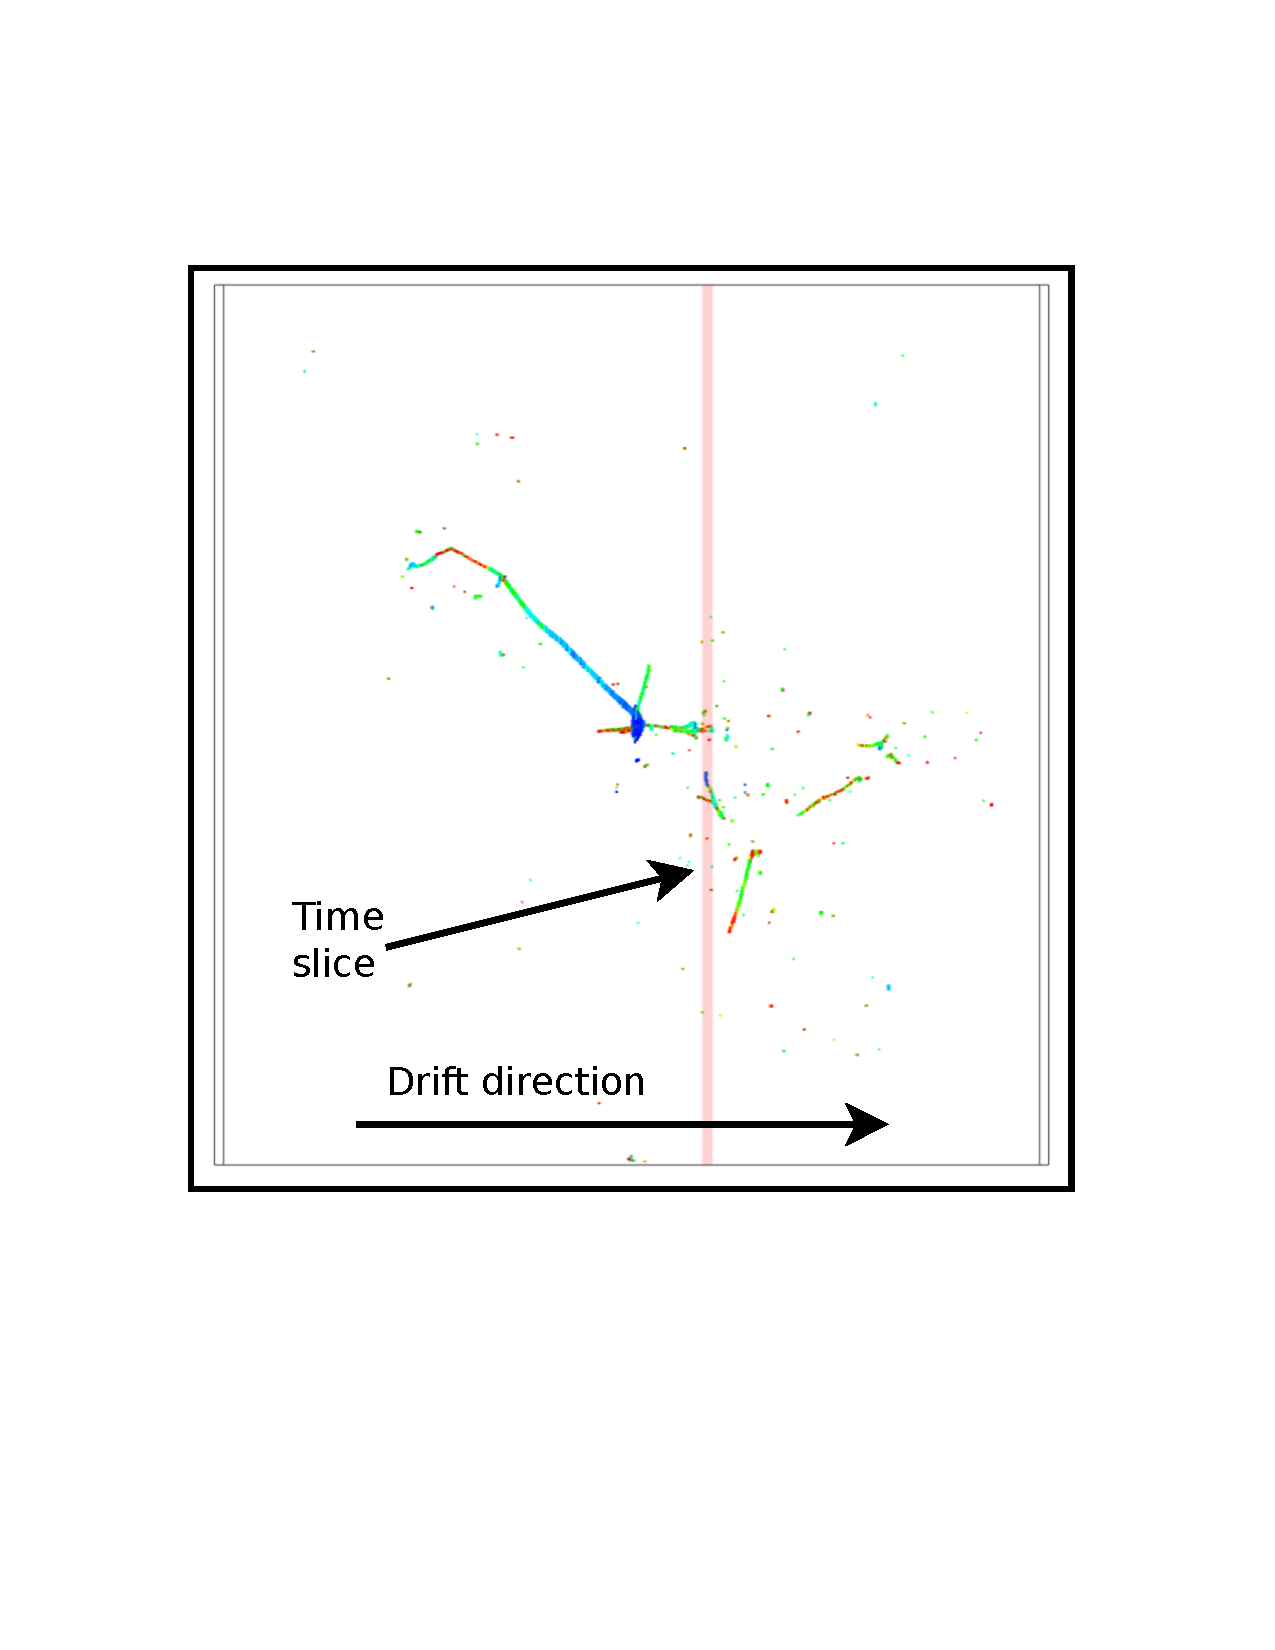
\includegraphics[width=\textwidth]{slice.pdf}

        \vspace{-2cm}

        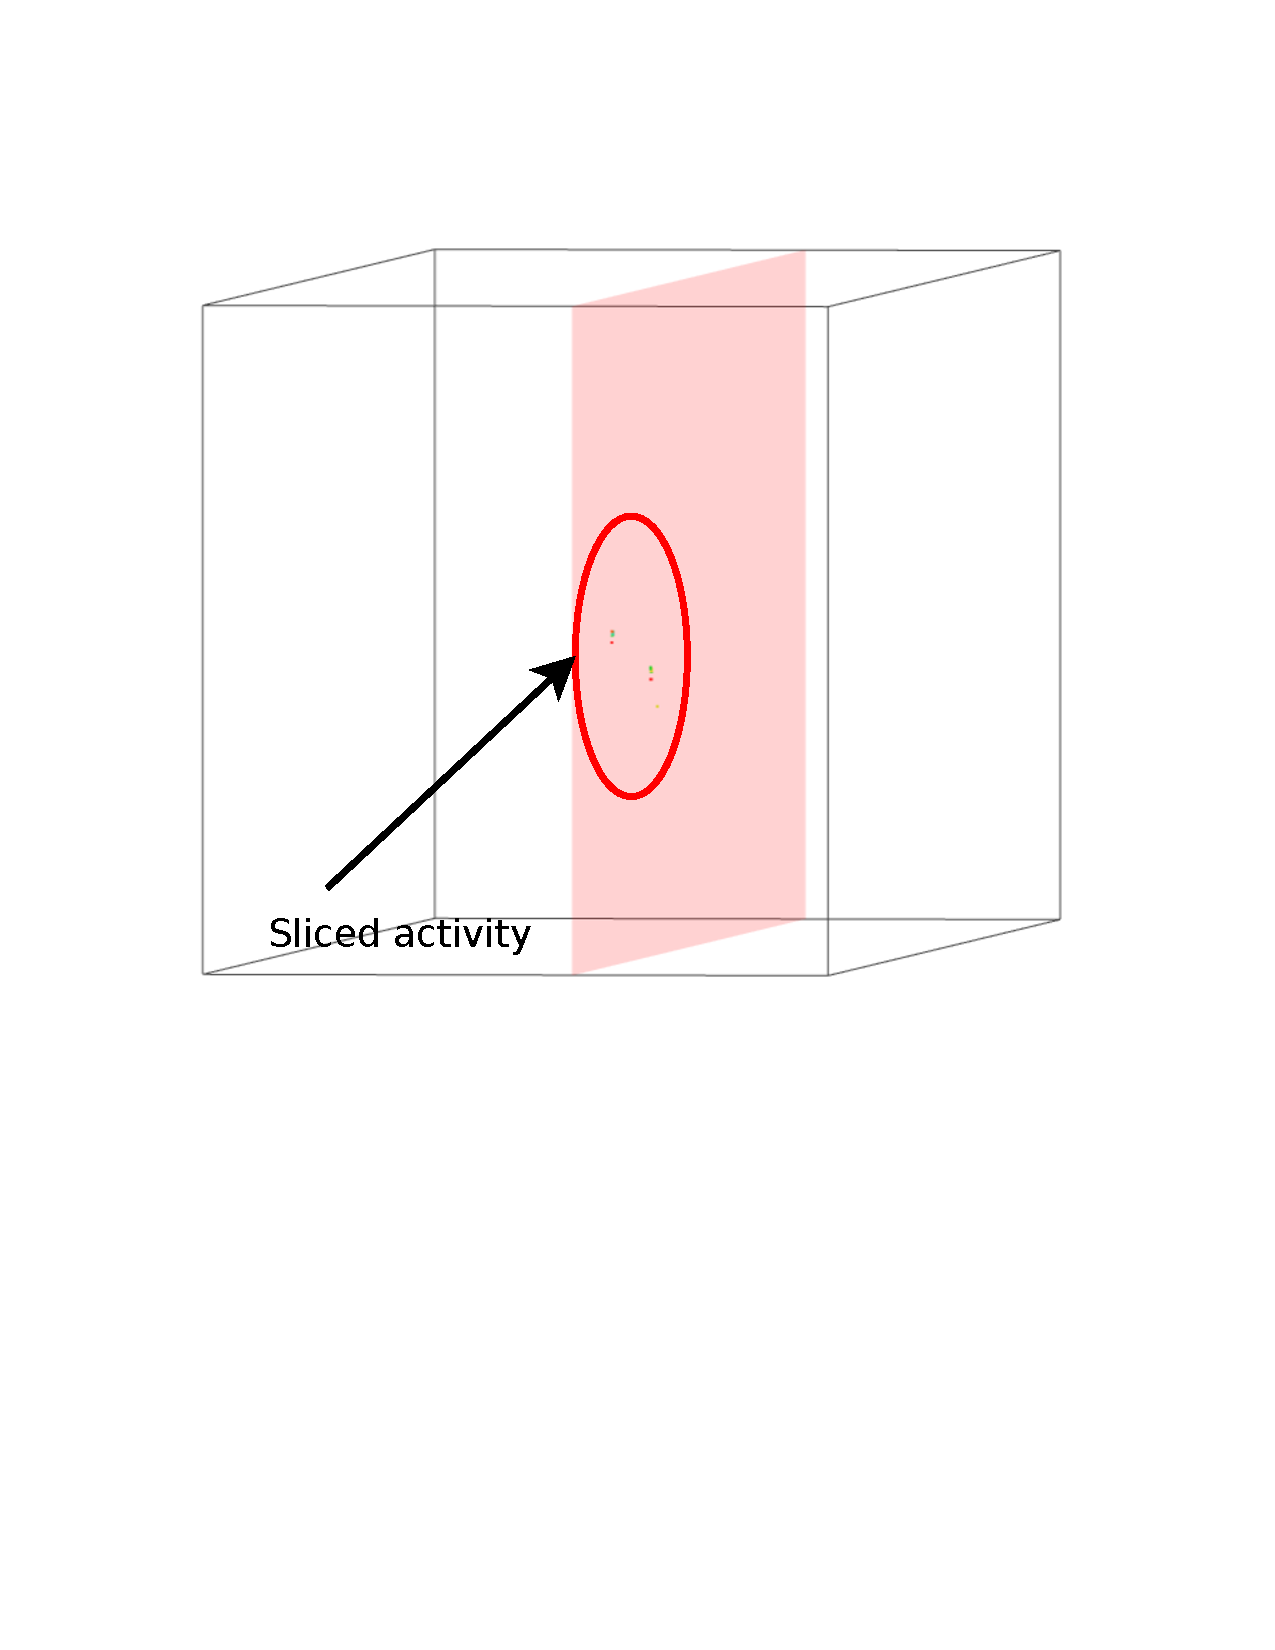
\includegraphics[width=\textwidth,trim=0cm 10cm 0cm 0cm,clip]{slice-3D.pdf}

        \scriptsize Focus on one \textbf{time slice} along a plane transverse to the drift.
      \end{center}
    \end{column}
    \begin{column}{0.65\textwidth}

      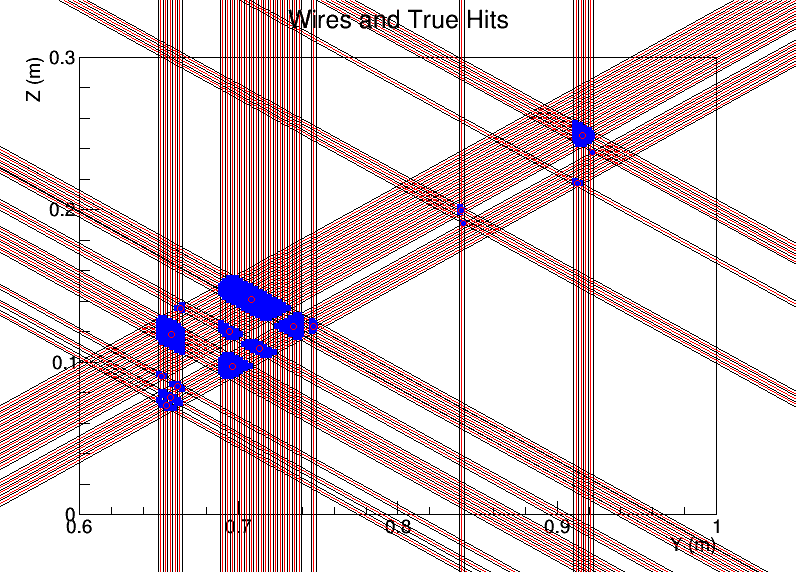
\includegraphics[width=0.9\textwidth]{wires-and-true-hits.png}

      \begin{itemize} \scriptsize
      \item Slice duration is chosen to \textbf{match
          electronics shaping time}: combine 4 FADC ``ticks'' =
        \SI{2}{\micro\second}.
      \item Select \textcolor{red}{wires} above threshold in the slice.
      \item Regions of triple-wire overlap: potential ``\textcolor{blue}{cells}'' holding charge in the \textbf{time slice}.
      \end{itemize}
    \end{column}
  \end{columns}

\end{frame}

\subsection{Imaging Of Activity}

\begin{frame}[fragile]
  \frametitle{Tiling}

  \vspace{-10mm}

  \begin{center}
    \scriptsize Zoom in on the wires and their associated (constructed) cells.

    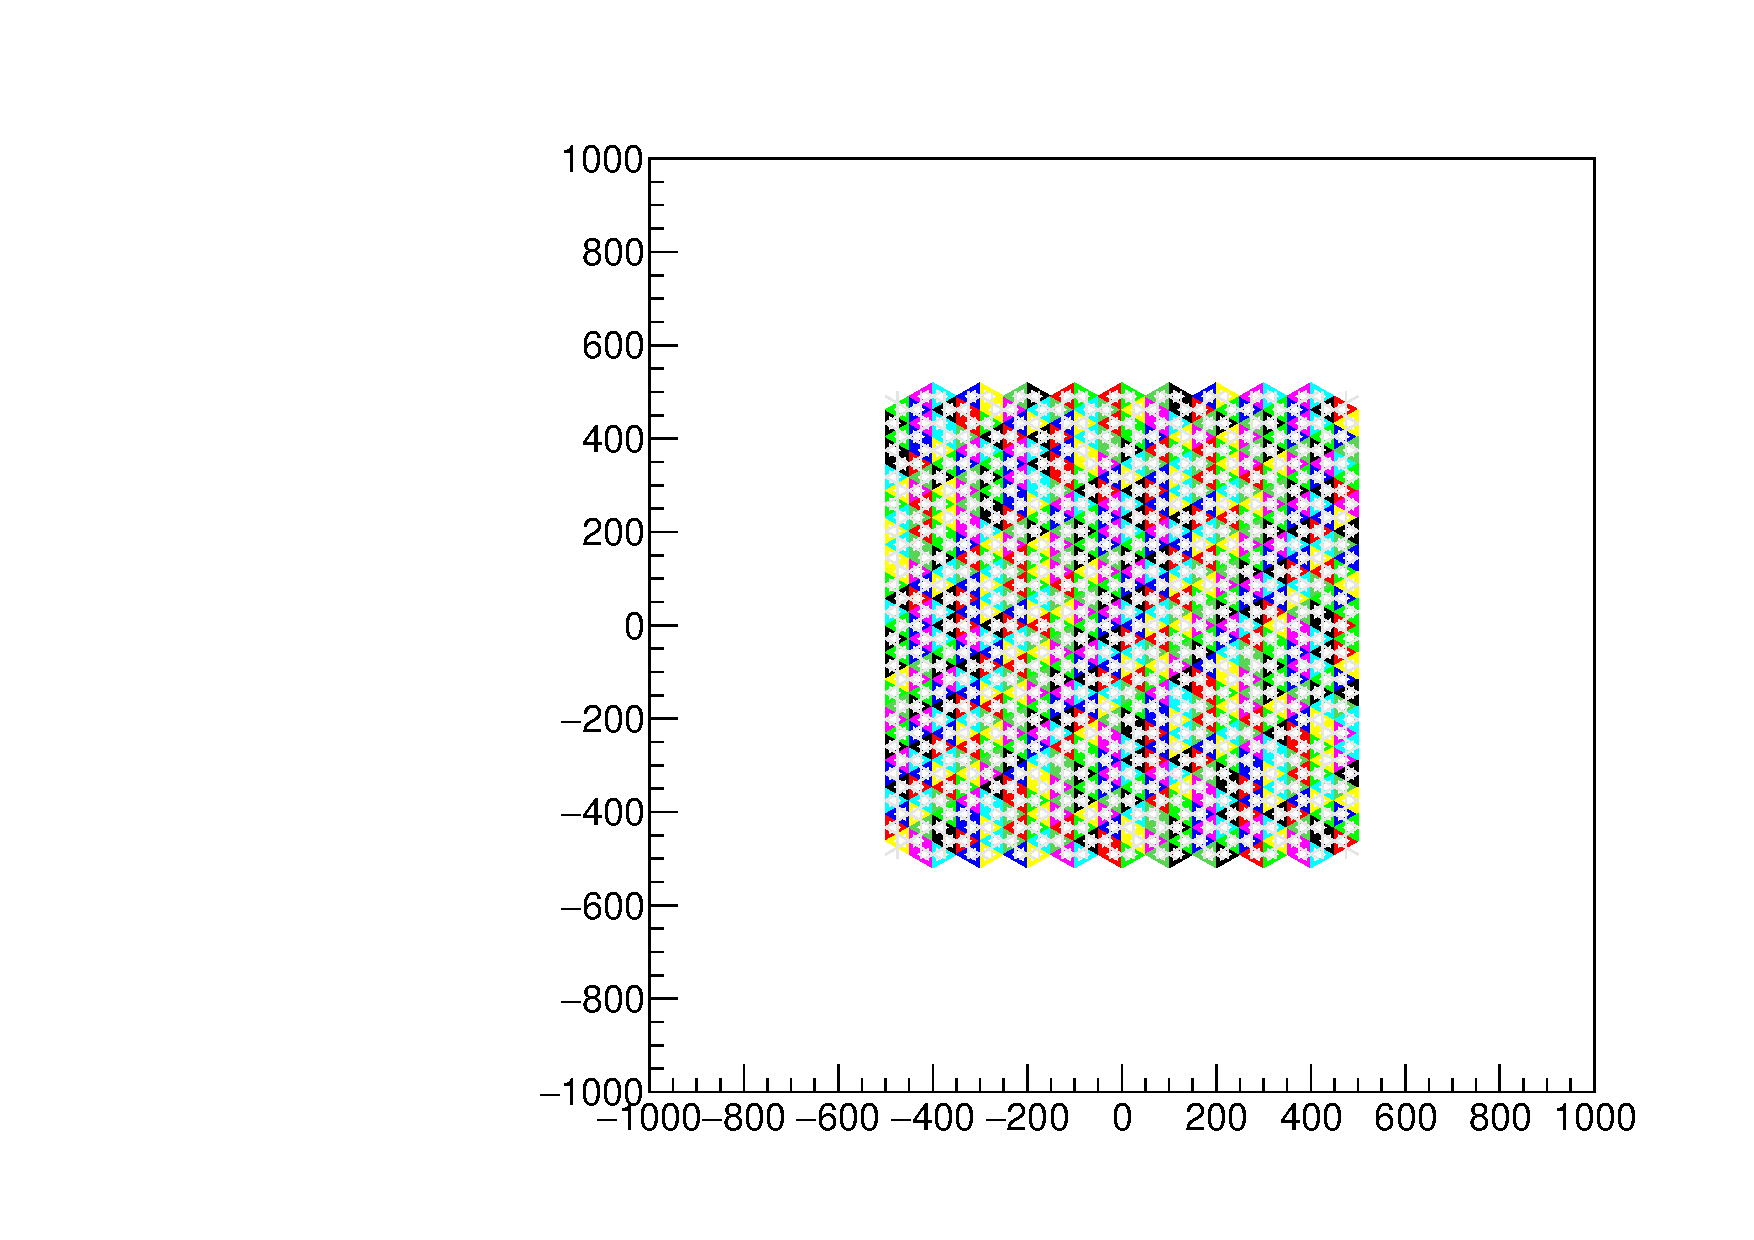
\includegraphics[width=0.7\textwidth,trim=8.6cm 10cm 8.6cm 9cm,clip]{test_boundcells_uboone.pdf}

    MicroBooNE geometry, grey wires, colored cells.
  \end{center}

  \footnotesize
  Cell construction:
  \begin{itemize}
  \item Each ``cell'' a 2D region near \textit{approximate triple crossings} of one wire from each of the three planes.
  \item Cells completely tile the plane.
  \item Cell pattern determined by wire \textbf{pitch}, \textbf{angle} and \textbf{phase}.
    \begin{description}
    \item[MicroBooNE] regular isosceles triangles.
    \item[DUNE] variety of polygons with a spectrum of sizes
    \end{description}
  \end{itemize}

  \textbf{The heart of the Wire Cell concept:} if all three of the
  triple-crossing \textbf{wires} are above threshold in a \textbf{time
    slice}, the associated \textbf{cell} likely contains the element
  of \textbf{drifted charge}.

\end{frame}

\begin{frame}
  \frametitle{Cell Ambiguity - Example Hit Pattern}

  \begin{columns}
    \begin{column}{0.35\textwidth}
      \begin{center}
        \scriptsize Zoom in on $5 \times 5 \times 3$ wires:

        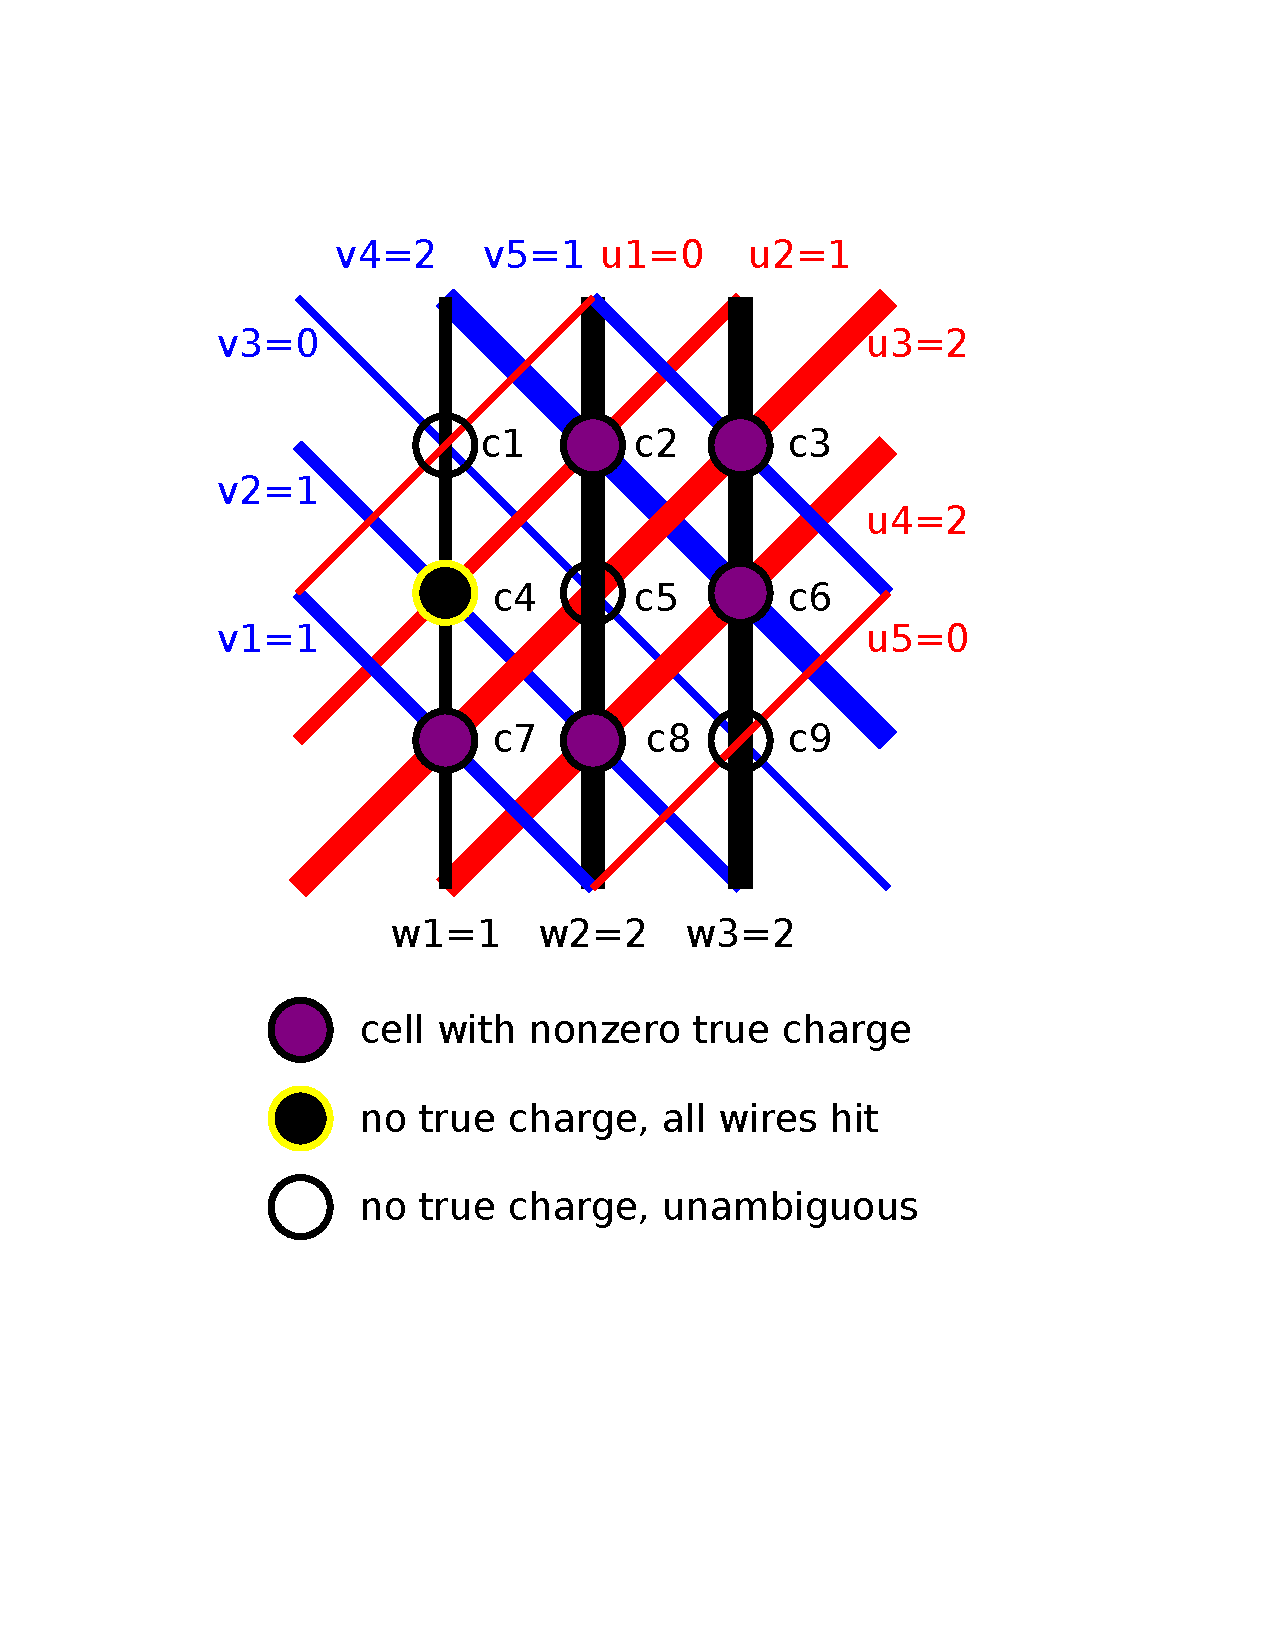
\includegraphics[width=\textwidth,trim=3.5cm 6cm 5cm 3cm,clip]{example-hit-cells.pdf}        

      \end{center}
    \end{column}
    \begin{column}{0.65\textwidth}

      Inherent \textbf{ambiguity} due to spatial multiplexing.

      \vspace{5mm}

      \begin{description}\scriptsize
      \item[Good] wire \textcolor{blue}{v3} measures no charge, \\$\therefore$ all its cells must \textbf{not} be hit.
      \item[Bad] hits \textbf{c2}, \textbf{c7} and \textbf{c8} induce ``ghost'' at \textbf{c4}.
      \item[Ambiguous] multiple cells measured by same wire.\\
        How much charge is in \textbf{c6}???
      \end{description}

      \vspace{5mm}

      \onslide<2->{
      Want to solve linear matrix equation like 
      \[\vec{w} = \mathbf{G} \vec{c}\]
    }
      \onslide<3>{\footnotesize{However, typical time slice has more \textbf{unknowns} (cells) than \textbf{knowns} (wires), ambiguities remain in solution}}.

    \end{column}
  \end{columns}
\end{frame}


\begin{frame}
  \frametitle{Blobs}
  \vspace{-10mm}
  \begin{columns}
    \begin{column}{0.6\textwidth}
      Goal: \textbf{reduce matrix size} and \textbf{remove ambiguity}.
    \end{column}
    \begin{column}{0.4\textwidth}
      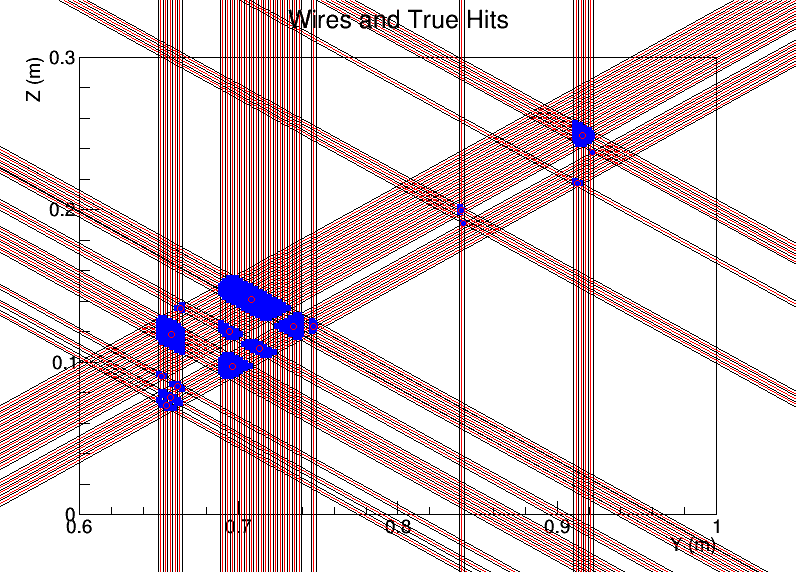
\includegraphics[width=0.8\textwidth]{wires-and-true-hits.png}          
    \end{column}
  \end{columns}
      
  \begin{enumerate}
  \item Select cells with their three wires above threshold.
  \item Partition set into spatially contiguous subsets: ``\textbf{blobs}''.
  \end{enumerate}
  Equation to solve becomes:
  \[\vec{w_b} = \mathbf{G_{wb}} \vec{b}\]

  \begin{description}
  \item[$\vec{b}$] vector of charge in each blob.
  \item[$\mathbf{G_{wb}}$] the wire-blob adjacency matrix for the slice.
  \item[$\vec{w_b}$] vector of charge on all wires associated with a blob.
  \end{description}

  Now, often \textbf{more favorable numerology}: $N_{blob} \lesssim N_{w_b}$
\end{frame}

% maybe remove this slide...
\begin{frame}
  \frametitle{Another wrinkle: charge uncertainty}

  Each wire's measure of drifting charge is uncertain.
  \begin{itemize}
  \item Environmental, electronic and thermal noise.
    \begin{itemize}\footnotesize
    \item[$\rightarrow$] Can be correlated across wires/channels/chips/boards/etc.
    \end{itemize}
  \item Statistical uncertainty due to digitization.
  \item Systematic uncertainties from deconvolution.
  \end{itemize}

  \vspace{3mm}

  Form a $\chi^2$ comparing measured wire charge ($\vec{w}_{meas}$)
  with expected ($\vec{w}_{exp}$) and covariance uncertainty matrix
  $\mathrm{V}$.
  
  \[\chi^2 = (\vec{w}_{meas}-\vec{w}_{exp})^\intercal\mathrm{V}^{-1} (\vec{w}_{meas}-\vec{w}_{exp})\]

  \vspace{3mm}

  \begin{center}
    \textbf{$\rightarrow$ This is a very CPU intensive, but critical step!}
  \end{center}

  \footnotesize And recall:
  \begin{itemize}
  \item this must be done at the raw-data processing stage
  \item need to do this each \SI{2}{\milli\second} time slice
  \end{itemize}

\end{frame}

\begin{frame}[fragile]
  \frametitle{The Payoff: imaged \SI{3}{\giga\electronvolt} $\nu_e$ interaction}
  
  \begin{columns}
    \begin{column}{0.5\textwidth}
      \begin{center}
        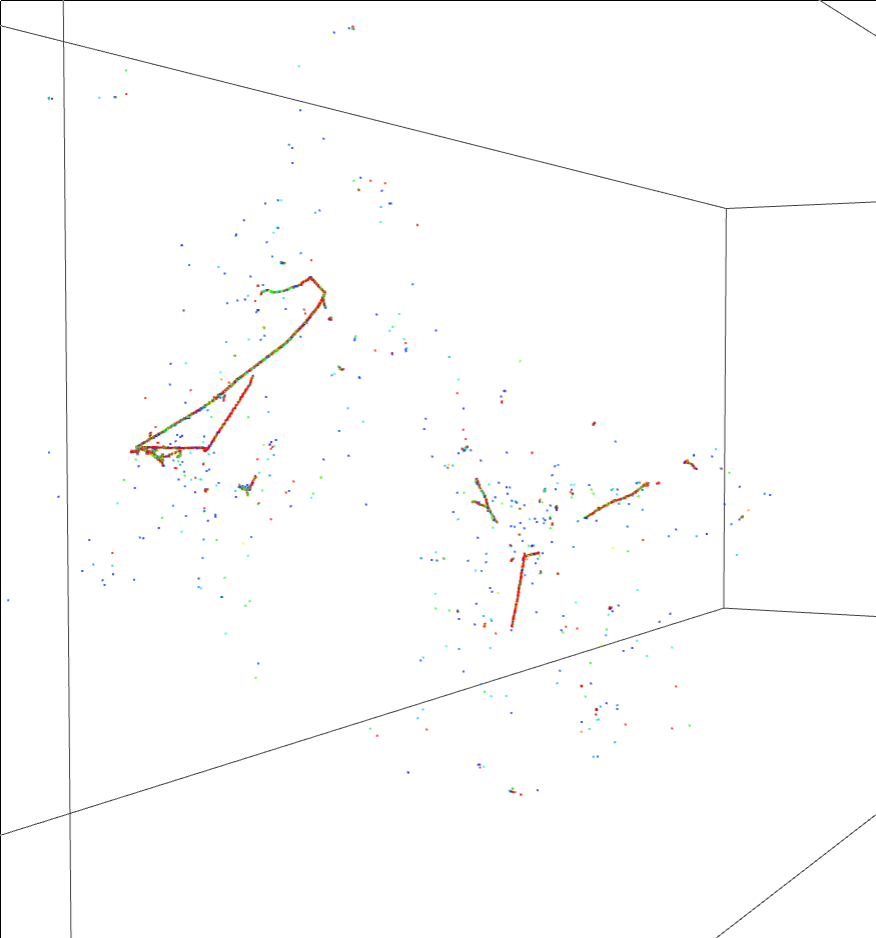
\includegraphics[width=\textwidth,trim=3cm 10cm 3cm 10cm,clip]{payoff-true.png}

        True energy depositions.
      \end{center}
    \end{column}
    \begin{column}{0.5\textwidth}
      \begin{center}
        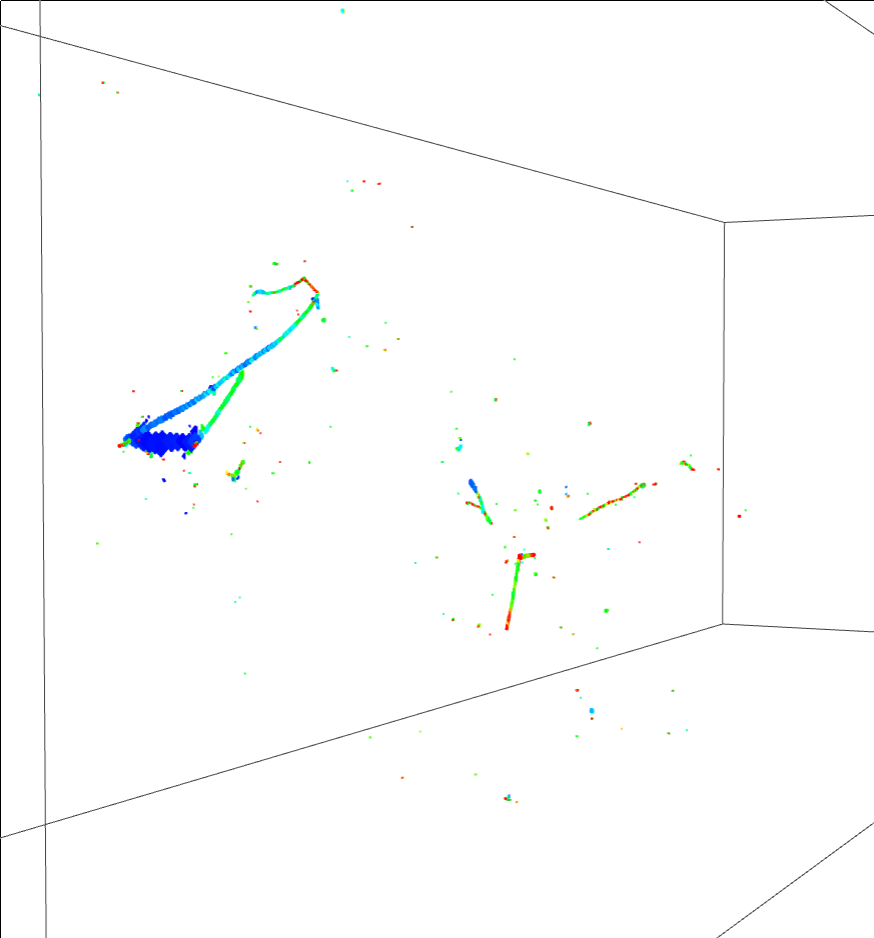
\includegraphics[width=\textwidth,trim=3cm 10cm 3cm 10cm,clip]{payoff-reco.png}

        Wire Cell Imaging.
      \end{center}
    \end{column}
  \end{columns}

  \vfill

  \footnotesize
  \begin{itemize}
  \item \textbf{Excellent imaging} of major track features as well as isolated
    activity.
    \begin{itemize}\scriptsize
    \item[$\rightarrow$] a static 2D view doesn't do it justice!  \href{http://www.phy.bnl.gov/wire-cell/bee/set/6/event/0/}{Follow link to try it}.
    \end{itemize}
  \item \textbf{Residual ambiguity} seen as wide blue patches.
    \begin{itemize}\scriptsize
    \item[$\rightarrow$] \textbf{Inherent in LArTPC technology}, Wire Cell just makes it evident.
      \begin{itemize}\scriptsize
      \item due to activity running parallel to the wire plane in one time slice.
      \end{itemize}
    \item[$\rightarrow$] Pursue
      an \textbf{iterative} approach: constrain ambiguous regions
      after taking well reconstructed parts to the kinematics-level.
    \end{itemize}
  \end{itemize}
\end{frame}


\subsection{Pattern Recognition}

\begin{frame}
  \frametitle{Pattern Recognition}
  Our current \textbf{post-imaging} approach:
  \begin{enumerate}
  \item \textbf{cluster} together blobs contiguous in space and time
    (slice).
  \item \textbf{track} a line through a cluster.
  \item \textbf{categorize} success/failure of track to account for the
    cluster's charge distribution.
  \end{enumerate}
  Some categories:
  \begin{description}
  \item[track] cluster is well characterized by the track.
  \item[shower] cluster consistent with an EM/hadronic shower.
  \item[short] cluster appears to be a ``short track'' (eg, $\delta$-ray).
  \item[undefined] no well-suited categorization.
  \end{description}

  \begin{itemize}
  \item This is an \textbf{active area of development} for Wire Cell.
  \item Maybe a problem suited for \textbf{machine learning}? 
  \end{itemize}

\end{frame}
